\subsection{Behaviour of Model under Parameter Changes}
\label{sec:og.param.effects}

To replicate the dynamics seen in the model, it is helpful to know, how the model changes along the areas of the same period.
\Cref{fig:yunus.function.evolution.12} shows, how the model function changes along the area of period 12.
In the figure, there are three functions in three different colors.
The first function is blue and it is the model with parameters $E_0 = 15.9, \chi_0 = 0.11$, it is marked as point $A_12$ in \Cref{fig:yunus.function.evolution.map}.
The second function is purple and it is the model at the point $E_0 = 17.07, \chi_0 = 0.182$, marked as point $B_{12}$.
The last function is red and it is the model with parameters $E_0 = 18.5, \chi_0 = 0.27$, marked as point $C_{12}$.

\begin{figure}
    \centering
    \begin{subfigure}{0.4\textwidth}
        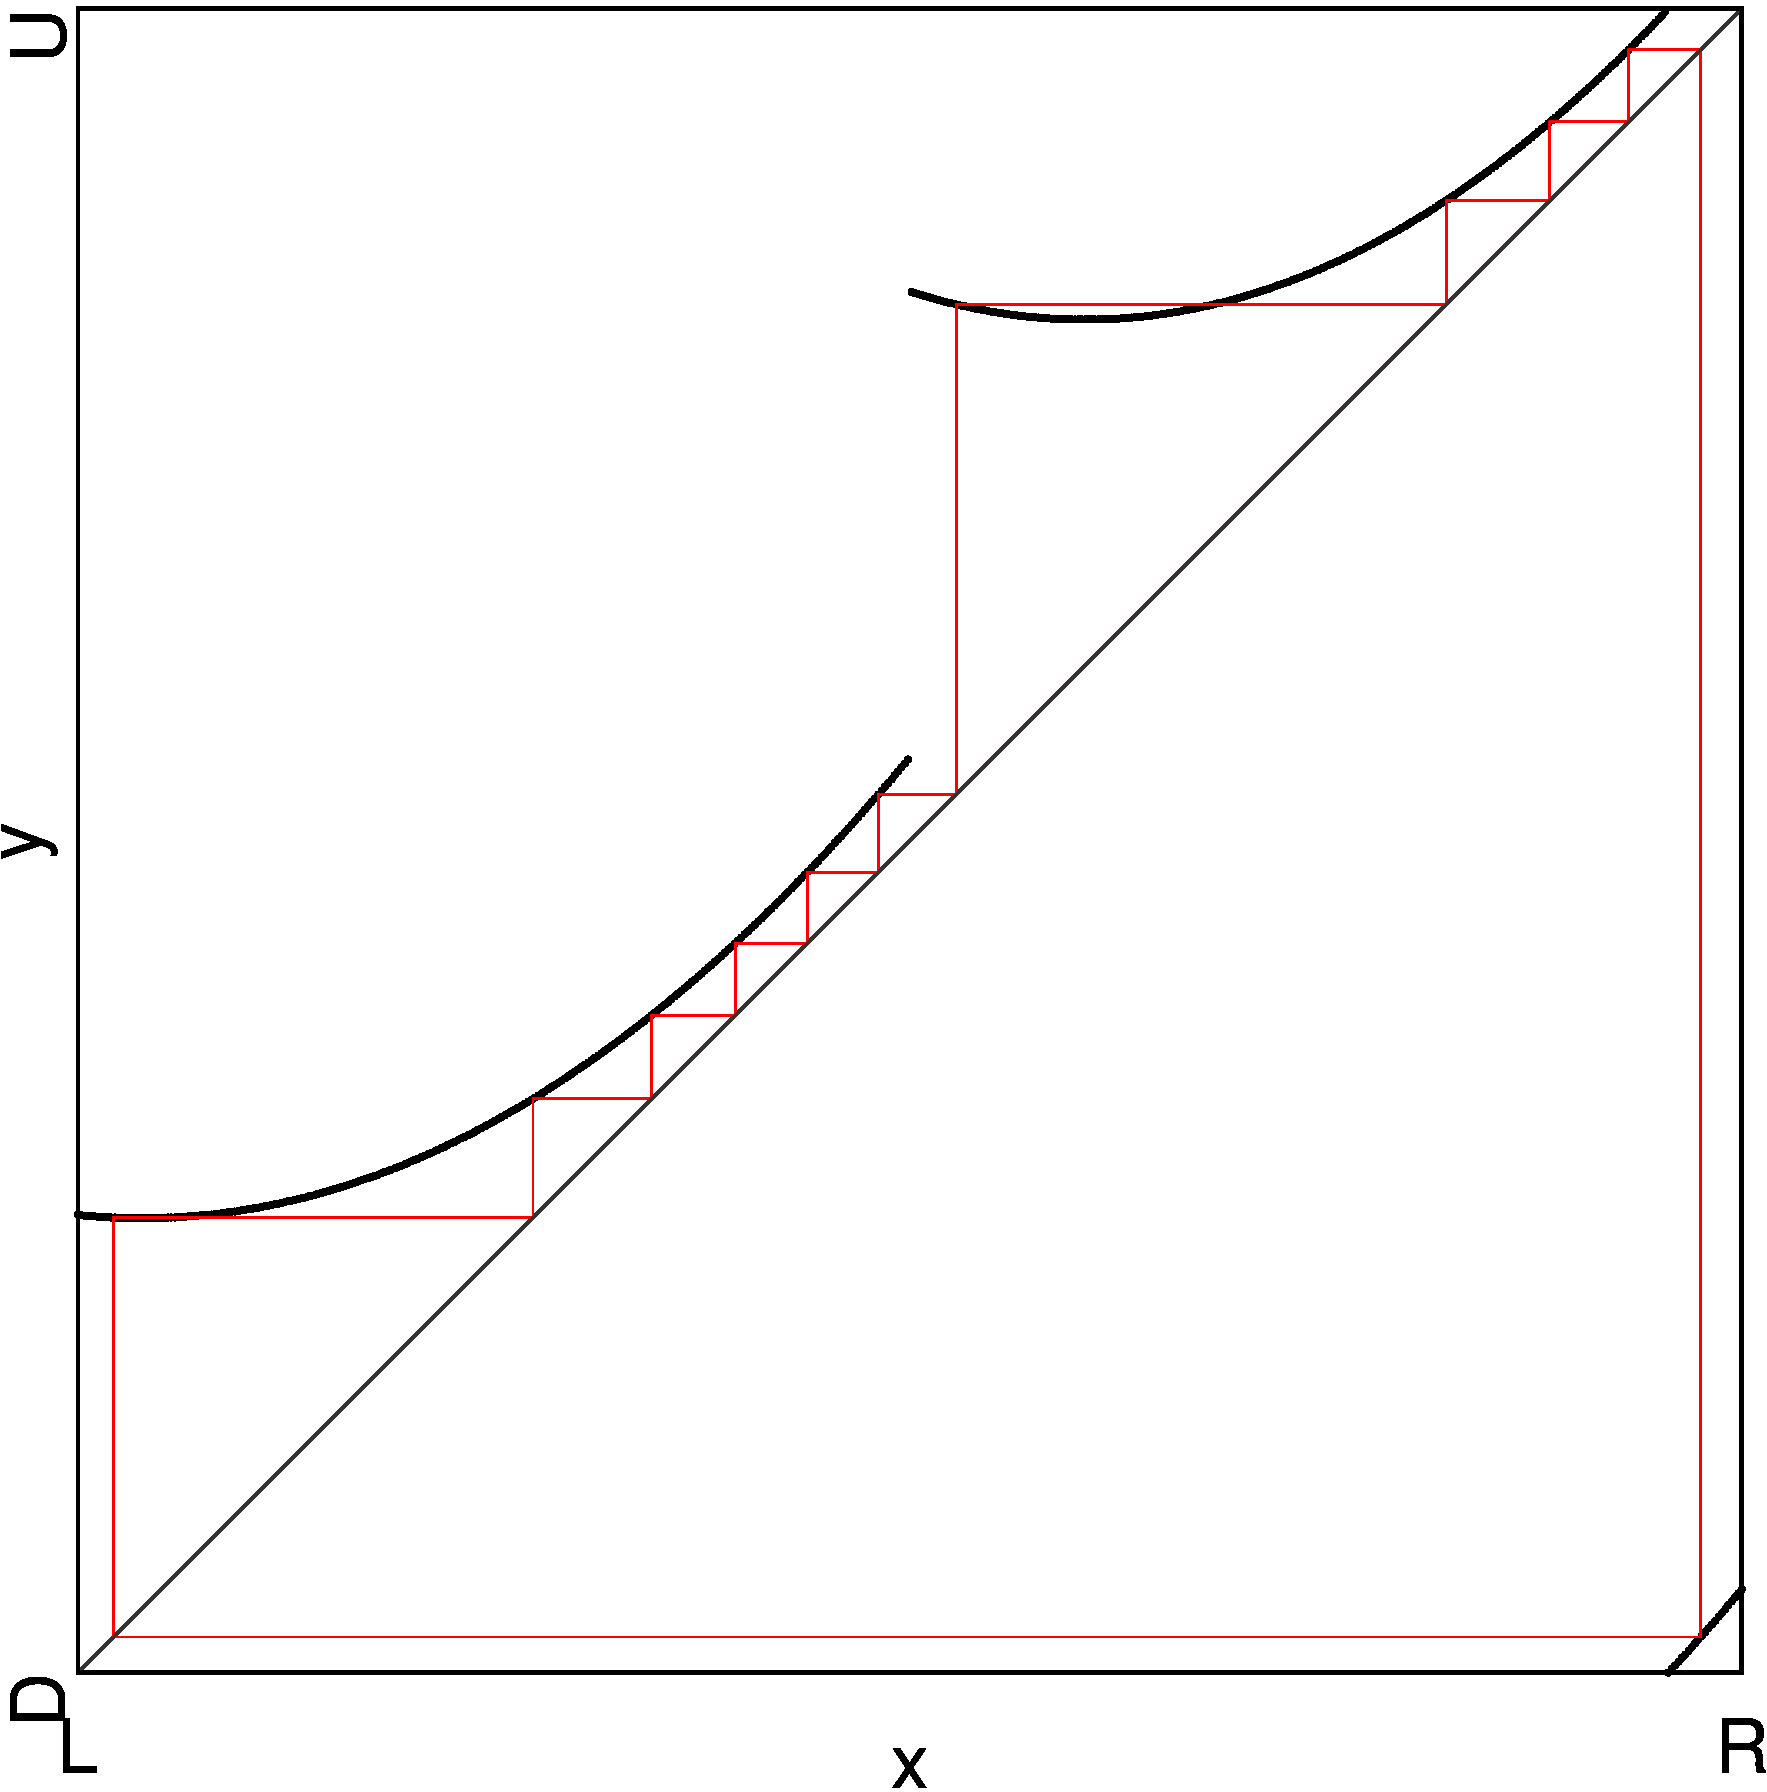
\includegraphics[width=\textwidth]{99_Yunus/2D_Period_Zoomed_Effects/result.png}
        \caption{Measured Points}
        \label{fig:yunus.function.evolution.map}
    \end{subfigure}
    \begin{subfigure}{0.4\textwidth}
        \includegraphics[width=\textwidth]{99_Yunus/ParameterEffects/E0_hi_P12/illustration.png}
        \caption{Evolution for Period 12}
        \label{fig:yunus.function.evolution.12}
    \end{subfigure}
    \begin{subfigure}{0.4\textwidth}
        \includegraphics[width=\textwidth]{99_Yunus/ParameterEffects/E0_hi_P10/illustration.png}
        \caption{Evolution for Period 10}
        \label{fig:yunus.function.evolution.10}
    \end{subfigure}
    \begin{subfigure}{0.4\textwidth}
        \includegraphics[width=\textwidth]{99_Yunus/ParameterEffects/E0_hi_P08/illustration.png}
        \caption{Evolution for Period 8}
        \label{fig:yunus.function.evolution.08}
    \end{subfigure}
    \caption{Effects of the Parameters on the Original Funtion}
\end{figure}

The most notable changes are
\begin{enumerate*}
    \item Branches $\A$ and $\C$ move upwards while the left part moves upwards more
    \item The left part of branches $\B$ and $\D$ move downwards 
    \item The local minima of these branches move to the left and downwards.
\end{enumerate*}
Smaller changes include
\begin{enumerate*}
    \item The border between branches $\B$ and $\C$ moves left
    \item The border between branches $\A$ and $\B$ moves right.
\end{enumerate*}
Note that regarding the borders, what happens to the border from $\B$ to $\C$, also applies to the border from $\D$ to $\A$.
Analogous for the borders from $\A$ to $\B$ and from $\C$ to $\D$ respectively.

The same effects can be observed for the areas of period 8 and 10.
The effects are visualized in \Cref{fig:yunus.function.evolution.10,fig:yunus.function.evolution.08}.
The points used for measurement are visualized in \Cref{fig:yunus.function.evolution.map}.
For the period 10, points $A_{10}, B_{10},$ and $C_{10}$ are used and for period 8, points $B_8$ and $C_8$.
